%%%%%%%%%%%%%%%%%%%%%%%%
%This tempelate is provided by Abdorrahman Mehri Ghahfarrokhi, petroleum university of technology, department of energy economics.
%email address: amehri.ghahfarrokhi@gmail.com
%%%%%%%%%%%%%%%%%%%%%%%%%

\RequirePackage[utf8]{inputenc}
\RequirePackage[T1]{fontenc}
\documentclass [xcolor=svgnames, t] {beamer} 
\usepackage[utf8]{inputenc}
\usepackage{booktabs, comment}
%\usepackage[slovak]{babel}
\usepackage[absolute, overlay]{textpos} 
\usepackage{pgfpages}
\usepackage[font=footnotesize]{caption}
\useoutertheme{infolines} 

\definecolor{red}{RGB}{250,0,75}
\setbeamercolor{title in head/foot}{bg=red, fg=white}
\setbeamercolor{author in head/foot}{bg=myuniversity}
\setbeamertemplate{page number in head/foot}{}
\usepackage{csquotes}


\usepackage{amsmath}
\usepackage[makeroom]{cancel}


\usepackage{textpos}

\usepackage{tikz}
\usepackage{algpseudocode}  % part of algorithmicx package
\usepackage{algorithm}

\usetheme{Madrid}
\definecolor{myuniversity}{RGB}{0, 85, 150}
\usecolortheme[named=myuniversity]{structure}
\usepackage{tikz}

\newtheorem{defn}{Definition}[section]
\newtheorem{thm}{Theorem}[section]
\newtheorem{claim}{Claim}[section]


\newtheorem{Shap}{Shapleyho hodnota}[section]
\newtheorem{Vektor}{\textbf{Vektorový prostor $\Gamma^n$}}[section]
\newtheorem{Trh}{Trh}[section]
\newtheorem{Obchod}{Obchod}[section]
\newtheorem{Volhra}{Volební hra}[section]

\newtheorem{Jednohlas}{\textbf{Shapleyho hodnota jednohlasných her}}[section]
\newtheorem{Jadro}{Jadro}[section]

\newtheorem{Lemke}{Lemke-Howson algorithm}[section]
\newtheorem{Nic}{}[section]
\def\QQ{\mathbb{Q}}
\def\RR{\mathbb{R}}
\def\ZZ{\mathbb{Z}}
\def\NN{\mathbb{N}}

\algnewcommand\algorithmicswitch{\textbf{switch}}
\algnewcommand\algorithmiccase{\textbf{case}}
\algnewcommand\algorithmicassert{\texttt{assert}}
\algnewcommand\Assert[1]{\State \algorithmicassert(#1)}%
% New "environments"
\algdef{SE}[SWITCH]{Switch}{EndSwitch}[1]{\algorithmicswitch\ #1\ \algorithmicdo}{\algorithmicend\ \algorithmicswitch}%
\algdef{SE}[CASE]{Case}{EndCase}[1]{\algorithmiccase\ #1}{\algorithmicend\ \algorithmiccase}%
\algtext*{EndSwitch}%
\algtext*{EndCase}%



\title[Min Cut-Path Problem]{Min Cut-Path Problem}
\institute[]{Pavol Jozef Šafárik University in Košice \\Faculty of Science\\ Institute of Computer Science}
\titlegraphic{
\includegraphics[height=1.95cm]{picture/logopfupjsf.jpg}}
\author[Norbert Micheľ]{
	\\ Mgr. Norbert Micheľ \\
    Supervisor:
    \\
    prof. RNDr. Gabriel Semanišin, PhD.
    }


\addtobeamertemplate{navigation symbols}{}{%
    \usebeamerfont{footline}%
    \usebeamercolor[fg]{footline}%
    \hspace{1em}%
    \insertframenumber/\inserttotalframenumber
}

\begin{document}
\begin{frame}
\maketitle
\end{frame}

%%%%%%%%%%%%%%%%%%%%%%%%%%%%
%\logo{
\includegraphics[scale=0.14]{upjs-logo.png}}

%%%%%%%%%%%%%%%%%%%%%%%%%%


\begin{frame}{Cut-Path}


\begin{defn}[Cut-Path]
Let \(G = (V, E)\) be a graph, and let \(u, v \in V\) be two distinct vertices. A cut-path between \(u\) and \(v\) is a set of edges \(S \subseteq E\) such that:
\begin{itemize}
    \item There exist subsets \(A, B \subseteq S\) where:
    \begin{itemize}
        \item \(A\) is a cut separating \(u\) and \(v\) (i.e., removing \(A\) disconnects \(u\) and \(v\)),
        \item \(B\) is a path connecting \(u\) and \(v\) (i.e., \(B\) forms a sequence of edges between \(u\) and \(v\)).
    \end{itemize}
\end{itemize}
\end{defn}


  \begin{figure}[H]
    \centering
    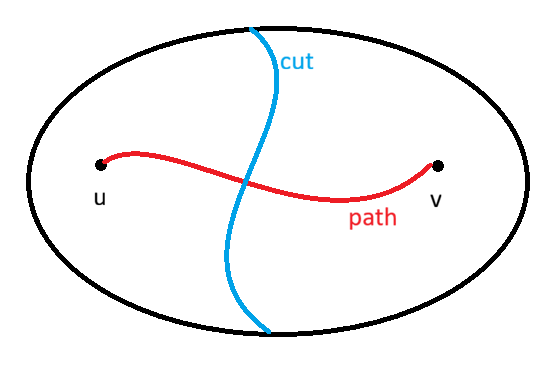
\includegraphics[width=60mm]{figures/obrazok_cut-path.png}   
    \label{fig:general_square_graph_pic}
\end{figure}
\end{frame}






\section{NP-Completeness of \textsc{Min Cut Path}}
















\begin{frame}{NP-Completeness of \textsc{Min Cut Path}}
\vspace{-0.7em}
\begin{thm}
The \textsc{Min Cut-Path} problem is NP-complete. 
\end{thm}

\vspace{0.2em}
\begin{itemize}
    \item \textbf{Reductions:}
    \begin{itemize}
        \item \textsc{3-SAT}
        \item $\downarrow$
        \item \textsc{Separating Shortest Path}
        \item $\downarrow$
        \item \textsc{Min Cut Path}
    \end{itemize}
\end{itemize}
\end{frame}

\begin{frame}{Separating Shortest Path}
\begin{problem}[\textsc{Separating Shortest Path}]
Let $G = (V,E)$ be an undirected graph and let $u,v \in V$ be two distinct vertices.  
A shortest $u$--$v$ path $P$ is called a \textsc{Separating Shortest Path} if the graph $G \setminus P$ contains no $u$--$v$ path.  
The \textsc{Separating Shortest Path} decision problem is defined as follows:

\begin{center}
\begin{tabular}{p{0.12\linewidth}p{0.8\linewidth}}
\textbf{Input:} & A graph $G = (V,E)$ and two distinct vertices $u,v \in V$.\\
\textbf{Question:} & Does there exist a shortest $u$--$v$ path in $G$ that is a separating shortest path?
\end{tabular}
\end{center}
\end{problem}
    
\end{frame}





\begin{frame}{NP-Completeness of \textsc{Min Cut Path}}
\vspace{-0.7em}
\begin{thm}
The \textsc{Min Cut-Path} problem is NP-complete. 
\end{thm}

\vspace{0.2em}
\begin{itemize}
    \item \textbf{Reductions:}
    \begin{itemize}
        \item \textsc{3-SAT}
        \item $\downarrow$
        \item \textsc{Separating Shortest Path}
        \item $\downarrow$
        \item \textsc{Min Cut Path}
    \end{itemize}
\end{itemize}
\begin{itemize}
    \item \textbf{Observation:}
    \begin{itemize}
        \item \textsc{Separating Shortest Path} $\rightarrow$ \textsc{Min Cut-Path} intuitive
    \end{itemize}
\end{itemize}
\end{frame}


\begin{frame}{Reduction from \textsc{3-SAT} to \textsc{Separating Shortest Path}}

    \begin{figure}[H]
    \centering
    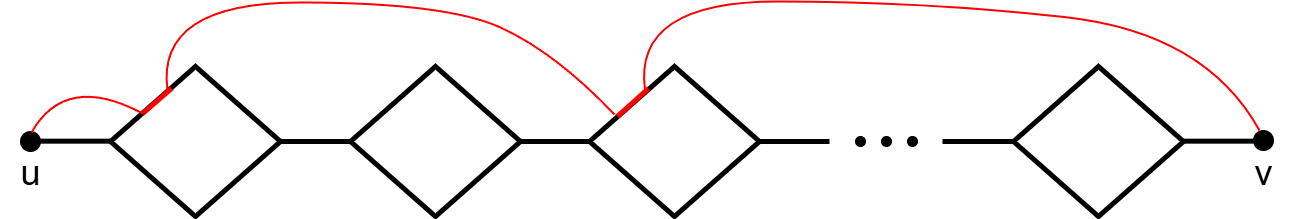
\includegraphics[width=120mm]{figures/chain_threads.png}   
    \label{fig:general_square_graph_pic}
\end{figure}

    \begin{itemize}
    \item Chain link
    \begin{itemize}
        \item Initialization chain link
        \item Terminal chain link
        \item Literal chain link
    \end{itemize}
        \item Thread 
        \begin{itemize}
            \item 2-synchronization thread
            \item 3-synchronization thread
            \item Clause thread
        \end{itemize}
    \end{itemize}

    
\end{frame}


\begin{frame}{Chain Link}

\begin{defn}[Chain Link]
Let $G=(V,E)$ be a graph and let $p,q \in V$ be two distinct vertices.  
A \emph{$(p,q)$-chain link} is a subgraph $L \subseteq G$ such that:
\begin{enumerate}
    \item $L$ is a simple cycle in $G$;
    \item the vertices $p$ and $q$ lie on $L$ and partition it into two internally disjoint $p$--$q$ paths;
    \item these two $p$--$q$ paths have equal length.
\end{enumerate}
\end{defn}

\begin{figure}[H]
    \centering
    
\includegraphics[width=50mm]{figures/chain_link.png}
    \label{fig:chain_link}
\end{figure}
\end{frame}




\begin{frame}{Chain}
\begin{definition}[Chain]
Let $G=(V,E)$ be a graph, and let $u,v\in V$.  
We say that $G$ is a \emph{$u$--$v$ chain} if the edge set $E$ can be partitioned into egde-disjoint subgraphs
\[
E = H_1 \cup L_1 \cup H_2 \cup L_2 \cup \cdots \cup H_m,
\]
where:
\begin{enumerate}
    \item each $H_i$ consists of a single edge with end-vertices $p_i,q_i$;
    \item each $L_i$ is a \emph{$q_i,p_{i+1}$-chain link}, i.e., a connected subgraph of $G$ with two distinguished end-vertices $q_i,p_{i+1}$;
    \item the first end-vertex $p_1$ coincides with $u$ and the last end-vertex of $H_m$ coincides with $v$.
\end{enumerate}
\end{definition}


\begin{figure}[H]
    \centering
    
\includegraphics[width=100mm]{figures/chain.png}
    \caption{\textbf{Chain}}
    \label{fig:chain}
\end{figure}
    
\end{frame}



\begin{frame}{Threading}
\begin{definition}[Threading]
Let $L$ be a chain link in a $u$--$v$ chain, and let $P$ be a thread not yet passing through $L$.  
The \emph{threading operation} on $(P,L)$ consists of the  this elementary operations:
\begin{enumerate}
    \item Select an edge $e=\{x,y\}$ of $L$ that is not used by any existing thread.
    \item Subdivide $e$ into a path $x$--$z_1$--$z_2$--$y$ of three edges, introducing two new vertices $z_1,z_2$.
    \item Extend $P$ so that it traverses the middle edge $\{z_1,z_2\}$ as its unique crossing of the chain link $L$.
\end{enumerate}


\end{definition}

\begin{figure}[H]
    \centering
    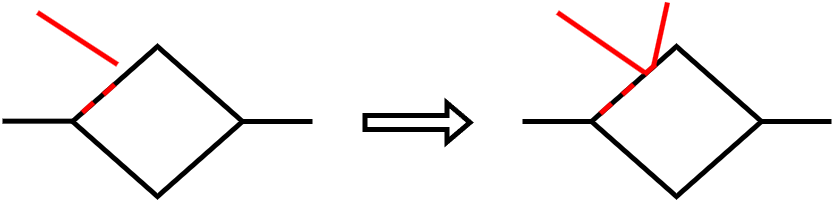
\includegraphics[width=100mm]{figures/Threading.png}
    \label{fig:Threading}
\end{figure}
    
\end{frame}

\begin{frame}{Chain link}

    Chain link
    \begin{itemize}
        \item Initialization chain link
        \item Terminal chain link
        \item Literal chain link
    \end{itemize}

    \begin{figure}[H]
    \centering
    
\includegraphics[width=100mm]{figures/Chain_link_example.png}
    \label{fig:Chain_link_example}
\end{figure}
\end{frame}

\begin{frame}{Thread}


Thread 
    \begin{itemize}
    \item 2-synchronization thread
    \item 3-synchronization thread
    \item Clause thread
\end{itemize}
\begin{figure}[H]
    \centering
    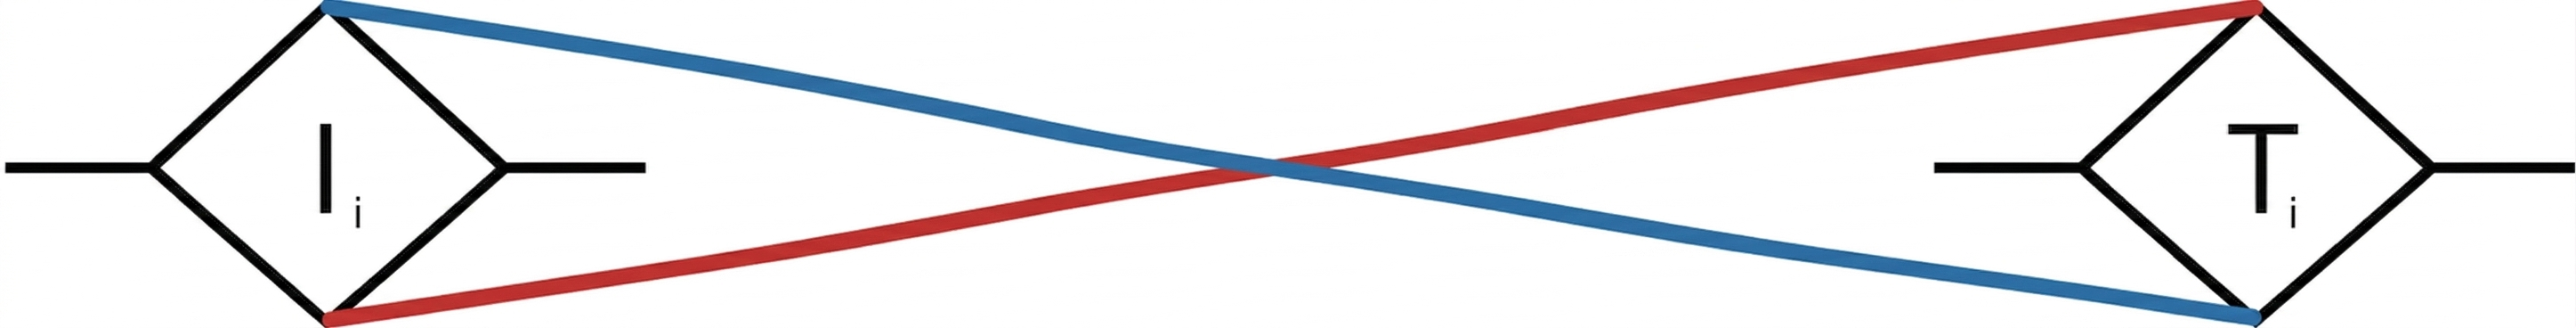
\includegraphics[width=100mm]{figures/2-sych.png}
    \label{fig:2-sych}
\end{figure}


\begin{figure}[H]
    \centering
    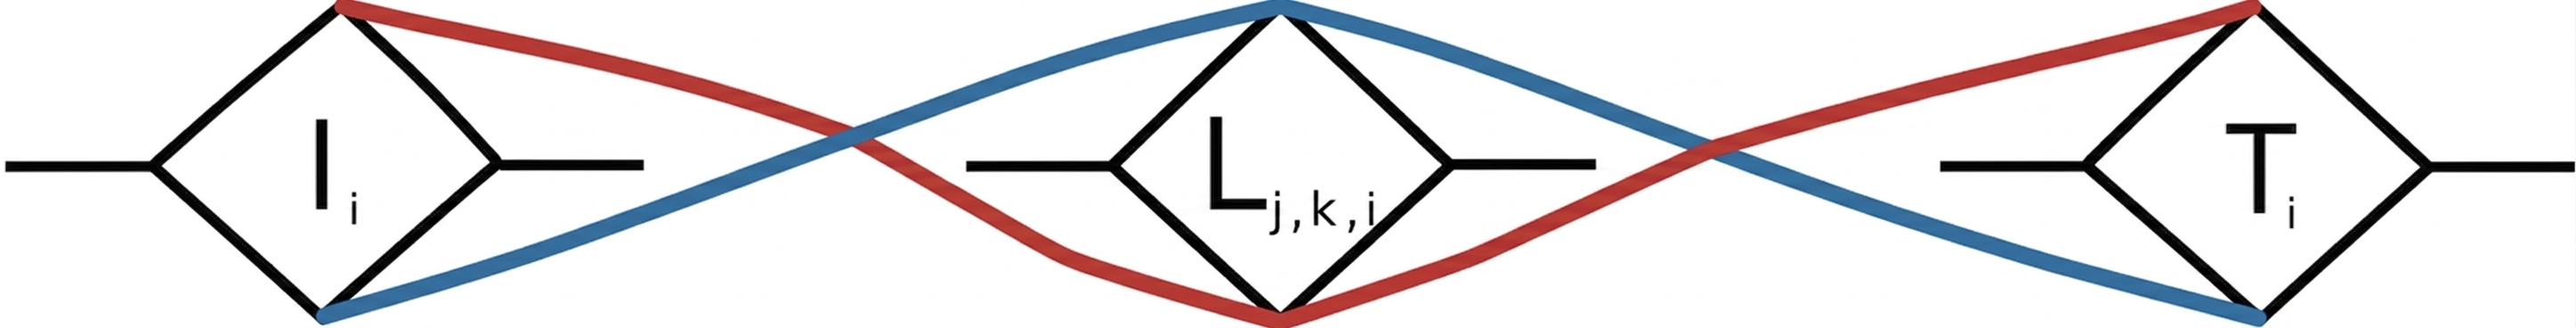
\includegraphics[width=100mm]{figures/3-sych.png}
    \label{fig:3-sych}
\end{figure}

\begin{figure}[H]
    \centering
    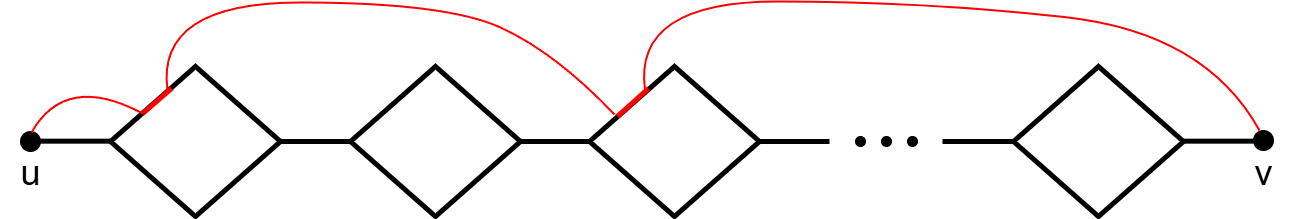
\includegraphics[width=100mm]{figures/chain_threads.png}   
    \label{fig:general_square_graph_pi}
\end{figure}


\end{frame}














\begin{frame}{Reduction from \textsc{3-SAT} to \textsc{Separating Shortest Path}}
\vspace{-1.8em}
\begin{algorithm}[H]
\tiny
\caption{Reduction from \textsc{3-SAT} to \textsc{Separating Shortest Path}}
\label{alg:reduction}
\begin{algorithmic}[1]
\Require Variables $X=\{x_1,\dots,x_n\}$, clauses $C=\{C_1,\dots,C_m\}$
\Ensure Graph $G$, vertices $u,v$
\State $n \gets |X|$, $m \gets |C|$
\State $G \gets \textsc{BuildChain}(u,v,2n+3m)$
\State $\mathcal{M} \gets$ map variable $\to$ list of literals
\For{$i \gets 1$ to $n$}
    \State $Lits \gets \mathcal{M}[x_i]$
    \State reserve $2+|Lits|$ chain links
    \State label first as $I_i$, last as $T_i$
    \For{each $\ell \in Lits$}
        \State assign next free link as $L_{\ell[0],\ell[1],i}$
    \EndFor
\EndFor
\For{$i \gets 1$ to $n$}
    \State $\textsc{Thread}(u,v,[(I_i,+),(T_i,-)])$
    \State $\textsc{Thread}(u,v,[(I_i,-),(T_i,+)])$
    \State $Lits \gets \mathcal{M}[x_i]$
    \For{each $\ell \in Lits$}
        \State $\textsc{Thread}(u,v,[(I_i,+),(L_{\ell[0],\ell[1],i},-),(T_i,+)])$
        \State $\textsc{Thread}(u,v,[(I_i,-),(L_{\ell[0],\ell[1],i},+),(T_i,-)])$
    \EndFor
\EndFor
\For{$i \gets 1$ to $m$}
    \State $\ell_1,\ell_2,\ell_3 \gets C_i$
    \State $\textsc{Thread}(u,v,[(L_{\ell_1[0],\ell_1[1]},s(\ell_1)),(L_{\ell_2[0],\ell_2[1]},s(\ell_2)),(L_{\ell_3[0],\ell_3[1]},s(\ell_3))])$
\EndFor
\State \Return $G$
\end{algorithmic}
\end{algorithm}
\end{frame}


\begin{frame}{Polynomial-time solvable islands}
\begin{itemize}
    
    \item \textbf{Polynomial-time solvable islands}
    \begin{itemize}
        \item Graphs of diameter two
        \item Graphs with minimum cut-value at most two
    \end{itemize}
    

\end{itemize}

  \begin{figure}[H]
    \centering
    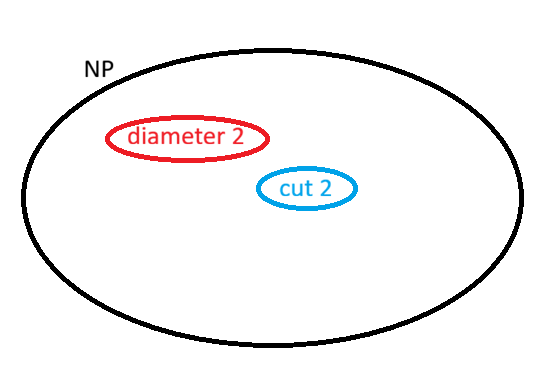
\includegraphics[width=60mm]{figures/triedy_zlozitosti.png}   
    \label{fig:general_square_graph_pic}
\end{figure}
\end{frame}










\section{Min Cut-Path Problem in Special Graph Classes}

\begin{frame}{Min Cut-Path Problem in Special Graph Classes}
\begin{thm}
Let \(G = (V, E)\) be a connected graph with diameter 2, and let \(u, v \in V\) be two distinct vertices. Then, the value of the min cut-path between \(u\) and \(v\) satisfies the following:
\[
cp(u, v) = c(u, v) + d(u, v) - 1.
\]
\end{thm}

\begin{thm}
\label{thm:min_cut_path_max_2}
Let \(G = (V, E)\) be a connected graph such that for every pair of distinct vertices \(x, y \in V\), the minimum cut satisfies:  
\[
c(x, y) \leq 2.
\]  
Then, the value of the min cut-path problem between \(u\) and \(v\) satisfies:
\[
cp(u, v) = c(u, v) + d(u, v) - 1.
\]
\end{thm}

\end{frame}



\section{Unification of polynomial-time islands}

\begin{frame}{Unification of polynomial-time islands}
\begin{itemize}
    \item \textbf{Motivation}
    \begin{itemize}
        \item Unification of polynomial-time islands
    \end{itemize}

    \item \textbf{Content}
    \begin{itemize}
        \item Unified class: \textbf{Diam-or-Cut-2}
        \item Decomposition of this class (\textbf{general square graph})
        \item Polynomial-time algorithm using general square graph decomposition
    \end{itemize}

\end{itemize}
  \begin{figure}[H]
    \centering
    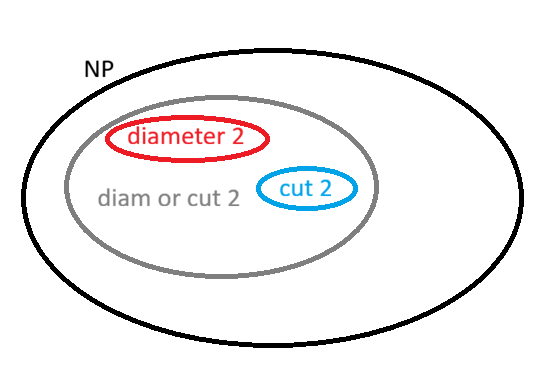
\includegraphics[width=60mm]{figures/triedy_zlozitosti_diam_or_cut-2.png}   
    \label{fig:general_square_graph_pic}
\end{figure}
\end{frame}


\begin{frame}{Diam or Cut 2 Graph}
\begin{defn}[Diam or Cut 2 Graph]
Let \(G = (V, E)\) be a graph. We say that \(G\) has the \textbf{diam or cut 2 graph} property if for every pair of distinct vertices \(x, y \in V\), at least one of the following conditions satisfies:
\[
c(x, y) \leq 2 \quad \text{or} \quad d(x, y) \leq 2.
\]  
\end{defn}
\begin{figure}[H]
    \centering
    \begin{minipage}{0.45\textwidth}
        \centering
        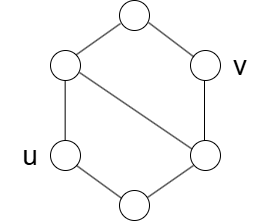
\includegraphics[width=35mm]{example_cut2.png}
        \subcaption{\textbf{\( c(u,v) = 2 \)}}
        \label{fig:example_cut2}
    \end{minipage}
    \hfill
    \begin{minipage}{0.45\textwidth}
        \centering
        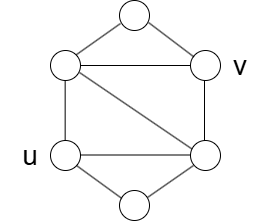
\includegraphics[width=35mm]{example_diam2.png}
        \subcaption{\textbf{\( d(u,v) = 2 \)}}
        \label{fig:example_diam2}
    \end{minipage}
    \caption{\textbf{Counterexample \( cp(u, v) \neq d(u, v) + c(u, v) - 1 \) }}
\end{figure}

\end{frame}


\begin{frame}{Diam or Cut 2 Graph}
\begin{defn}[Diam or Cut 2 Graph]
Let \(G = (V, E)\) be a graph. We say that \(G\) has the \textbf{diam or cut 2 graph} property if for every pair of distinct vertices \(x, y \in V\), at least one of the following conditions satisfies:
\[
c(x, y) \leq 2 \quad \text{or} \quad d(x, y) \leq 2.
\]  
\end{defn}
\begin{figure}[H]
    \centering
    \begin{minipage}{0.45\textwidth}
        \centering
        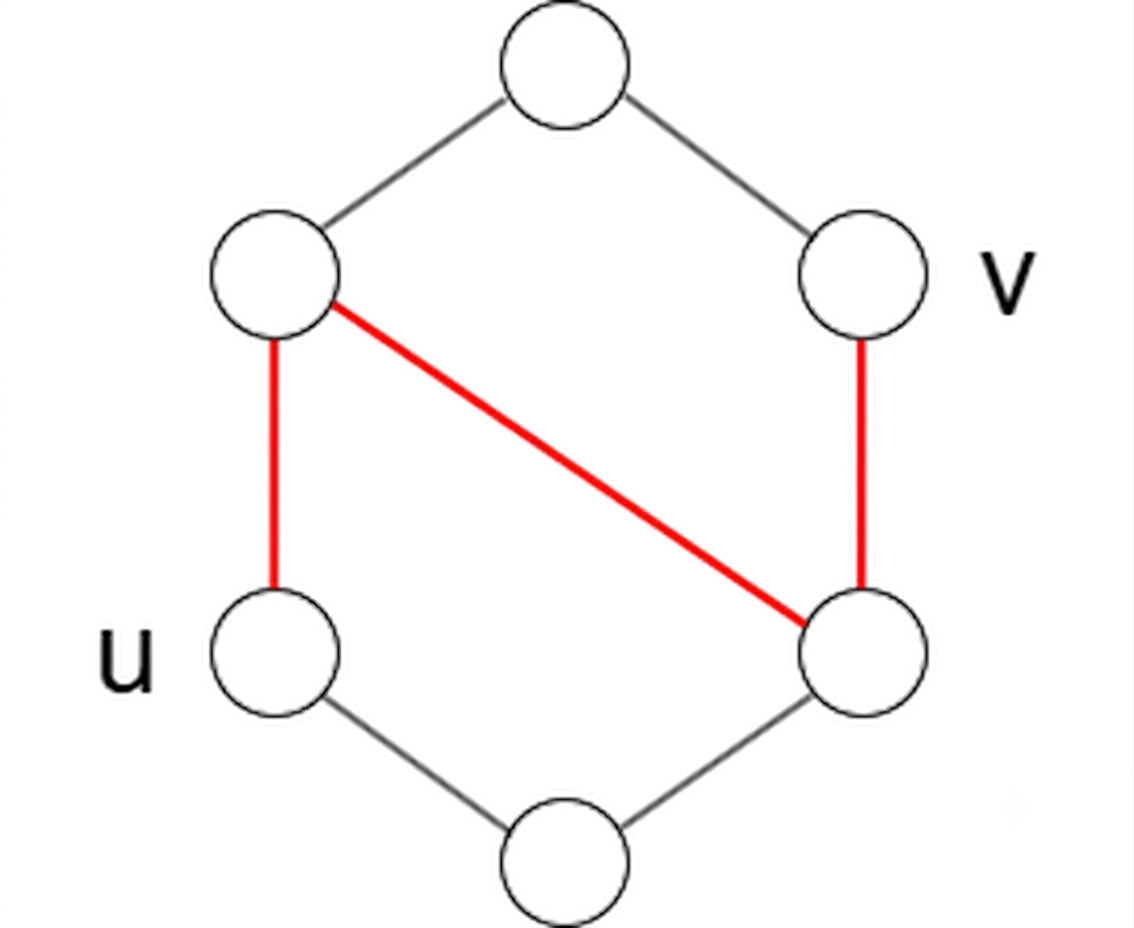
\includegraphics[width=35mm]{example_cut2c.png}
        \subcaption{\textbf{\( c(u,v) = 2 \)}}
        \label{fig:example_cut2c}
    \end{minipage}
    \hfill
    \begin{minipage}{0.45\textwidth}
        \centering
        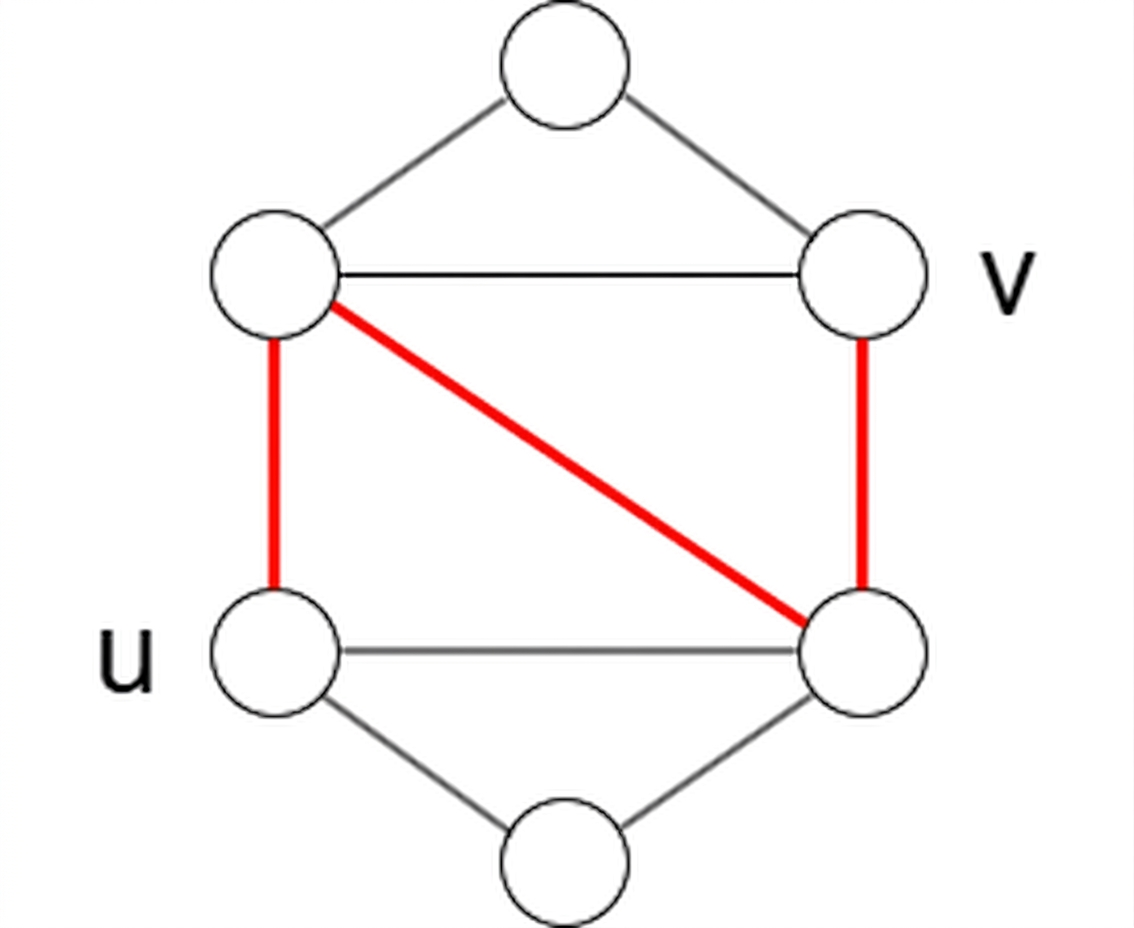
\includegraphics[width=35mm]{example_diam2c.png}
        \subcaption{\textbf{\( d(u,v) = 2 \)}}
        \label{fig:example_diam2c}
    \end{minipage}
    \caption{\textbf{Counterexample \( cp(u, v) \neq d(u, v) + c(u, v) - 1 \) }}
\end{figure}

\end{frame}








\begin{frame}{General Square Graph}
    \begin{figure}[H]
    \centering
    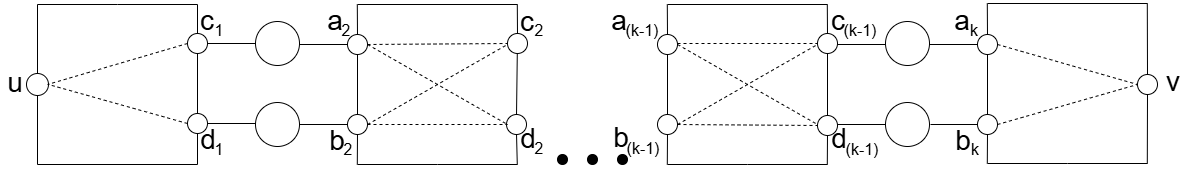
\includegraphics[width=120mm]{general_square_graph.png}   
    \label{fig:general_square_graph_pic}
\end{figure}
\end{frame}

\begin{frame}{Transformations}
\vspace{-0.8em}
\begin{figure}[H]
    \centering
    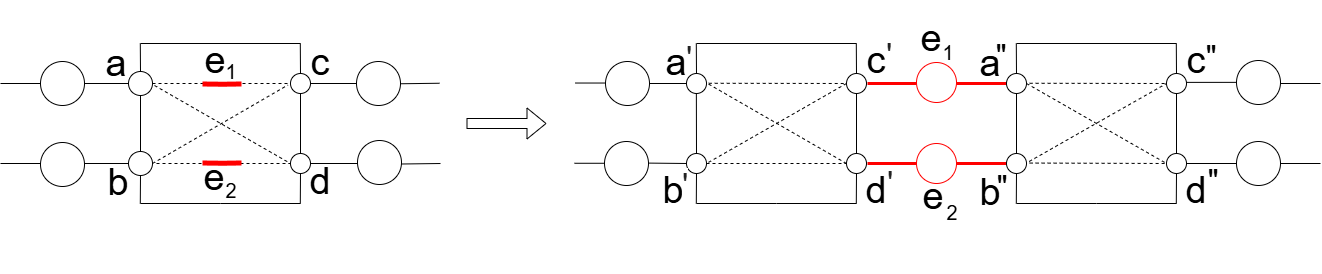
\includegraphics[width=120mm]{Transformation_A.png}
    \label{fig:Transformation_A}
\end{figure}

\vspace{-2.8em}
\begin{figure}[H]
    \centering
    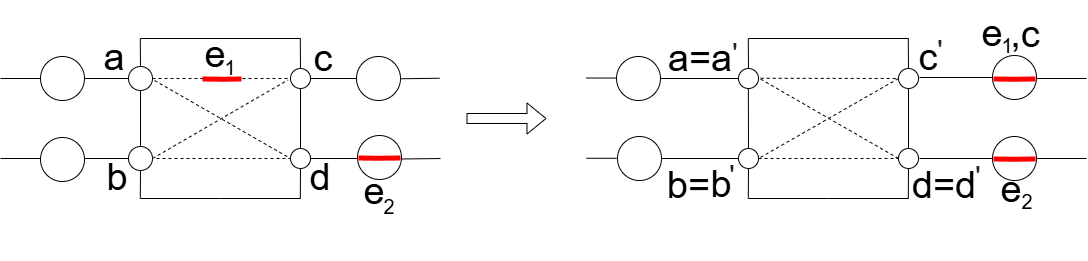
\includegraphics[width=100mm]{Transformation_B.png}
    \label{fig:Transformation_B}
\end{figure}

\vspace{-0.8em}
\begin{figure}[H]
    \centering
    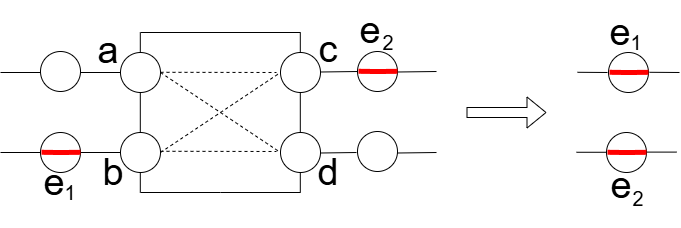
\includegraphics[width=70mm]{Transformation_C.png}
    \label{fig:Transformation_C}
\end{figure}
    
\end{frame}








\begin{frame}{Constructing a General Square Graph Decomposition}
\vspace{-1em} 
\begin{algorithm}[H]
\tiny
\label{alg:square_graph_revised}
\begin{algorithmic}[1]
\Require Graph \(G=(V,E)\) with property diam or cut 2, vertices \(u,v \in V\) such that \(c(u,v)=2\)
\Ensure A decomposition G into a valid square general graph between \(u\) and \(v\).

\State Initialize pseudo-square graph \(S_{initial}\) with \(a=u, b=u, c=v, d=v\) and \(V=V(G)\).
\State \(e_1, e_2 \leftarrow\) min \(cut(u, v)\)
\State \(S'_1, S'_2 \leftarrow\) TransformationA(\(G,S_{initial},e_1, e_2,u,v\)). 
\State Initialize \(S \leftarrow \{S'_1, S'_2\}\).

\While{\(S\) is not empty}
    \State \(S_{work} \leftarrow\) select and remove pseudo-square graph from \(S\).
    \For{each pair \((x, y)\) in \(\{(a, c), (b, d), (a, d), (b, c)\}\)}
        \If{\(d(x, y) > 2\)} \Comment{Checking if a pseudo-square graph is a square graph}
            \State \(e_1, e_2 \leftarrow\) min \(cut(x, y)\) \Comment{Edges \(e_1\) and \(e_2\) are within \(S_{work}\) intesection general paths that connects to this pseudo-square graph.}
            \State \(Count \leftarrow count(e_1, e_2 \in S_{work})\)
            \Switch{\(Count\)}
                \Case{0}
                    \State TransformationC(\(G,S_{work},e_1, e_2,x,y\))
                \EndCase
                \Case{1}
                    \State \(S'_1 \leftarrow\) TransformationB(\(G,S_{work},e_1, e_2,x,y\))
                    \State Add \(S'_1\) to \(S\).
                \EndCase
                \Case{2}
                    \State \(S'_1, S'_2 \leftarrow\) TransformationA(\(G,S_{work},e_1, e_2,x,y\))
                    \State Add \(S'_1, S'_2\) to \(S\).
                \EndCase
            \EndSwitch
            \State \textbf{break}
        \EndIf 
    \EndFor
\EndWhile
\State \textbf{Return} the constructed general square graph.
\end{algorithmic}
\end{algorithm}
    
\end{frame}


\begin{frame}{Polynomial-time algorithm}
\vspace{-1em}
    \begin{algorithm}[H]
    \tiny
\caption{Polynomial-time algorithm for computing \(cp(u,v)\) in a graph with the \textbf{diam or cut 2} property and \(c(u,v) = 2\)}
\begin{algorithmic}[1]
\Require Graph \(G=(V,E)\) with property diam or cut 2, vertices \(u,v \in V\) such that \(c(u,v)=2\)
\Ensure Value of \(cp(u,v)\)

\State Compute \(d(u,v)\) using breadth-first search
\State Construct the \textit{general square graph} \(H\) from \(G\) on vertices \(u,v\)
\State \(S \gets \emptyset\)
\ForAll{square graphs \(S_i\) in \(H\)}
    \State \(S \gets S \cup \{S_i\}\)
\EndFor

\ForAll{\(S_i \in S\)}
    \ForAll{possible vertex pairs \((x,y)\)}
        \State \(\{\alpha, \beta\} \gets\) the remaining two vertices of \(S_i\)
        \State \(P \gets\) the set of all shortest paths \(\leq2\) between \(x\) and \(y\)\Comment{We compute the shortest path within the square graph \(S_i\).}
        \ForAll{\(p \in P\)}
            \If{\(\alpha\) and \(\beta\) are in different components after removing the edges of path \(p\)}
                \State \(res \gets d(u,x) + d(x,y) + d(y,v)\)
                \If{\(res = d(u,v)\)}
                    \State \Return \(d(u,v)\)
                \EndIf
            \EndIf
        \EndFor
    \EndFor
\EndFor
\State \Return \(d(u,v) + 1\)
\end{algorithmic}
\end{algorithm}
\end{frame}












\begin{frame}{Thank You}
\vspace{1.5em}
\begin{center}
    \Large Thank you for your attention
\end{center}
\end{frame}










\end{document}
